\subsection{CR Alternativi:
CyberRangeCZ}\label{cr-alternativi-cyberrangecz}

\textbf{CyberRangeCZ} e\textquotesingle{} un fork di \textbf{KYPO}.
E\textquotesingle{} una piattaforma basata su OpenStack per fornire
un\textquotesingle ambiente cloud su cui fare il deploy delle macchine.
Utilizza tecnologie moderne come container, IaC (infrastructure as code)
ed i microservizi.

Macchine virtuali, reti, e training sono definiti utilizzando JSON e
YAML. Questi file vengono passati ad Ansible per descrivere il contenuti
della macchina e ad Packer per costruire le immagini delle macchine
virtuali.

Fa uso massivo della virtualizzazione per ricreare fedelmente reti
complesse ed interi sistmi operativi.

La piattaforma si concentra per soddisfare due casi
d\textquotesingle uso principali:

\begin{itemize}
\tightlist
\item
  emulare intere infrastrutture di computer in ambienti controllati
\item
  eseguire più sessioni di training contemporaneamente, gestendo
  centinaia di ambienti virtuali per centinaia o migliaia di
  partecipanti.
\end{itemize}

La piattaforma CyberRangeCZ si occupa di creare e approvvigionare
un\textquotesingle ambiente virtuale emulato costituito da Sandbox e
Pool.

\begin{quote}
\textbf{Sandbox}: \emph{"È un ambiente di test isolato con reti virtuali
che consente agli utenti di connettersi alle macchine virtuali (VM) e
comunicare con il resto della rete, la macchina host e le altre VM.
Sulle VM, l\textquotesingle utente può eseguire programmi, utilizzare
servizi di rete o monitorare il traffico di rete, il tutto senza
influire sull\textquotesingle infrastruttura esterna. La sandbox viene
eseguita all\textquotesingle interno del cloud ed è accessibile da
remoto."} \footnote{\label{fn:ref_13}\url{https://docs.platform.cyberrange.cz/basic-concepts/terminology/\#emulated-virtual-environment}}
\end{quote}

\begin{quote}
\textbf{Pool}: \emph{"Un gruppo di sandbox cloud create a partire dalla
medesima sandbox definition."} \footref{fn:ref_13}
\end{quote}

All\textquotesingle interno di una sandbox e\textquotesingle{} possibile
fornire una \textbf{Topology Definition}, un file che decsrive la
struttura dell\textquotesingle ambiente (host, router, reti, etc.)
mentre il \textbf{Sandbox Provisioning} si occupa di customizzare le
instanze nella topologia.


\begin{figure}[htbp]
  \centering
  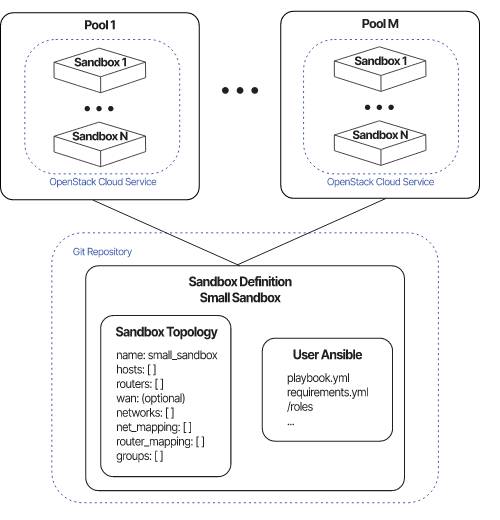
\includegraphics[width=0.92\linewidth,height=0.7\textheight,keepaspectratio]{src/images/KYPO-basic-elements-sandboxes.png}
  \caption{Kypo Basic Elements Sandboxes}
  \label{fig:KYPO-basic-elements-sandboxes}
\end{figure}


La creazione di una Sandbox si divide in 3 fasi:

\begin{itemize}
\tightlist
\item
  \textbf{Allocazione}: creazione della sandbox (=macchine virtuali)
  dentro al cloud.
\item
  \textbf{Networking}: setup della rete e distirbuzione delle chiavi di
  accesso dentro le macchine.
\item
  \textbf{Provisioning}: customizzazione delle macchine virtuali nella
  sandbox.
\end{itemize}

\begin{quote}
La creazione della Pool precede necessariamente la creazione delle
Sandbox.
\end{quote}

A partire dalla Topology Definition, viene prodotta la \textbf{Topology
Instance} utilizzando \passthrough{\lstinline!Terraform!} (che crea
l\textquotesingle infrastruttura virtuale). L\textquotesingle accesso
alla topologia e\textquotesingle{} regolato da un MAN (Management Access
Node), ossia l\textquotesingle unico nodo connesso
all\textquotesingle esterno della rete della Topology Instance.

Di seguito, nell\textquotesingle immagine sburgoz, viene mostrata
l\textquotesingle architettura generale di una Topology Instance.

\begin{figure}[htbp]
  \centering
  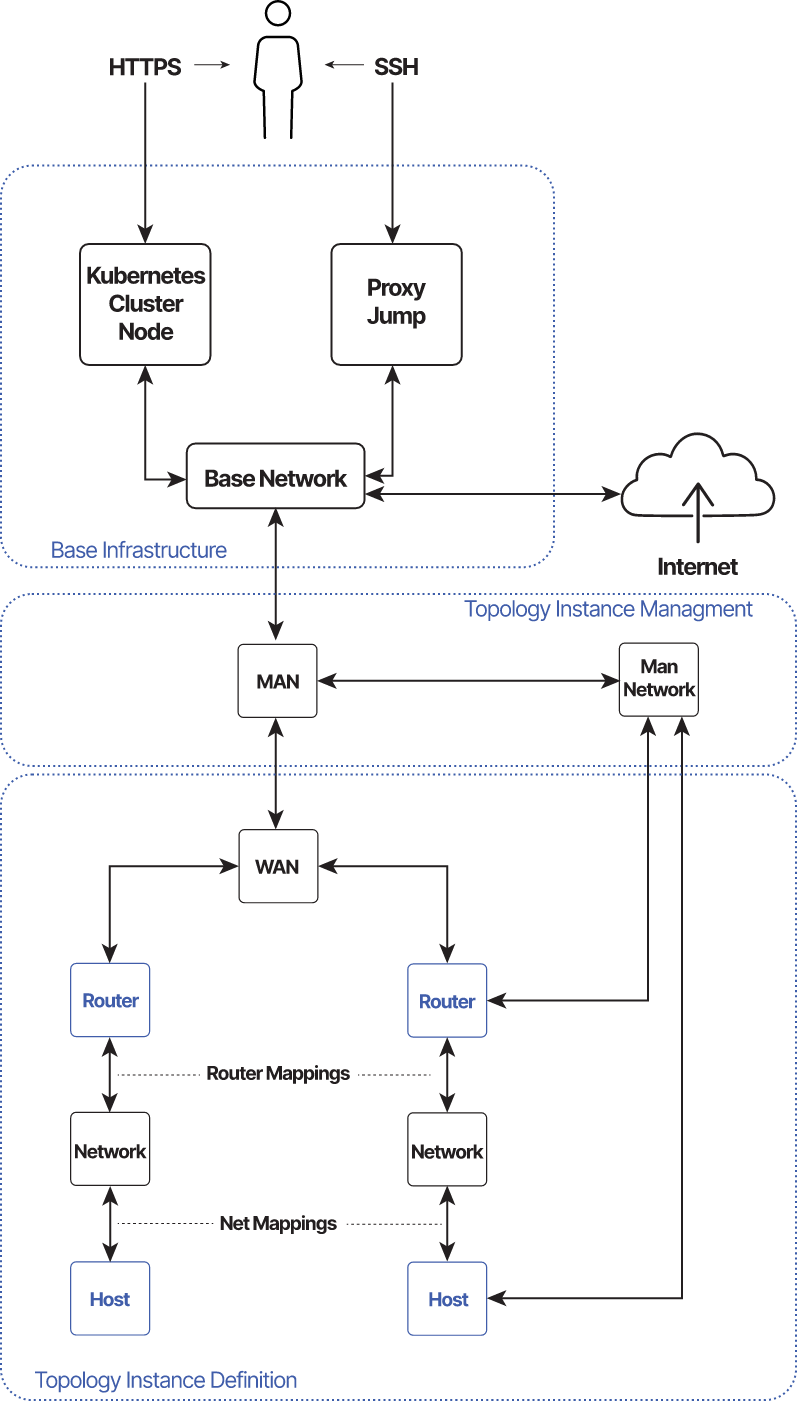
\includegraphics[width=0.92\linewidth,height=0.7\textheight,keepaspectratio]{src/images/KYPO-topology-instance.png}
  \caption{Kypo Topology Instance}
  \label{fig:KYPO-topology-instance}
\end{figure}


L\textquotesingle accesso alle macchine dentro la Sandbox
e\textquotesingle{} regolato tramite SSH, oppure da una console web
accessibile via browser.

Gestire Sandobx, ossia intere Topology Instance e\textquotesingle{}
costoso, infatti i requisiti sono i seguenti:

\begin{itemize}
\tightlist
\item
  una macchina virtuale con almeno \emph{2 core CPU, 16 GB di RAM e 40
  GB di archiviazione}
\item
  un server dotato di almeno \emph{16 core CPU, 128 GB di RAM, 2 TB di
  archiviazione e almeno due interfacce di rete.}
\end{itemize}

Requisiti cosi alti sono necessari per:

\begin{itemize}
\tightlist
\item
  gestire l\textquotesingle infrastruttura OpenStack, i microservizzi, e
  Kubernetes
\item
  gestire l\textquotesingle esecuzione di centinaia di macchine virtuali
  e garantire la scalabilita al crescere degli utenti. Si consideri che
  uno scenario base potrebbe per esempio richiedere 4 CPU virtuali, 4 GB
  di RAM e 41 GB di disco. Per 30 partecipanti si arriva a consumare gia
  1.2TB di spazio sul disco.
\end{itemize}

Quindi CyberRangeCZ e\textquotesingle{} un software complesso e
flessibile che si applica a molti scenari, tutta via, non si applica al
nostro problema orignale poiche:

\begin{itemize}
\tightlist
\item
  Creare un\textquotesingle intera topologia richiede
  l\textquotesingle uso di piu tool tra cui Ansible, alzando
  all\textquotesingle ordine dei minuti il tempo per il provisioning
  della Sandbox.
\item
  Non e\textquotesingle{} previsto un meccanismo di verifica dello stato
  delle macchine come discusso in \textbf{1.2}
\item
  Inoltre, i requisiti di minimi sono eccessivi e si potrebbe pensare
  anche di migliorare questo aspetto.
\end{itemize}
